\documentclass[11pt, a4paper]{article}
\usepackage{a4wide,amsmath,amsfonts,graphicx,subcaption,tikz}
\usepackage[spanish]{babel}
%\usepackage[ruled,vlined]{algorithm2e}

%\parindent = 0 pt
\parskip = 5 pt

\newcounter{row}
\newcounter{col}

\newcommand\setrow[3]{
	\setcounter{col}{1}
	\foreach \n in {#1, #2, #3} {
	\edef\x{\value{col} - 0.5}
	\edef\y{3.5 - \value{row}}
	\node[anchor=center] at (\x, \y) {\n};
	\stepcounter{col}
	}
	\stepcounter{row}
}

\newcommand\setrowaux[7]{
	\setcounter{col}{1}
	\foreach \n in {#1, #2, #3, #4, #5, #6, #7} {
	\edef\x{\value{col} - 0.5}
	\edef\y{7.5 - \value{row}}
	\node[anchor=center] at (\x, \y) {\n};
	\stepcounter{col}
	}
	\stepcounter{row}
}

\newcommand{\real}{\mathbb{R}}

\begin{document}
\begin{center}
\begin{tabular}{r|cr}
 \begin{tabular}{c}
{\large\bf\textsf{\ M\'etodos Num\'ericos\ }}\\ 
Primer Cuatrimestre 2015\\
{\bf Trabajo Pr\'actico 3}\\
\end{tabular} &
\begin{tabular}{@{} p{1.6cm} @{}}

\includegraphics[width=1.6cm]{logodpt.jpg}
\end{tabular} &
\begin{tabular}{l @{}}
 \emph{Departamento de Computaci\'on} \\
 \emph{Facultad de Ciencias Exactas y Naturales} \\
 \emph{Universidad de Buenos Aires} \\
\end{tabular} 
\end{tabular}
\vskip 10pt
\textbf{\Large \emph{Marche un telebeam Don Niembraaaaaa...}}\\
\vspace{0.5cm}
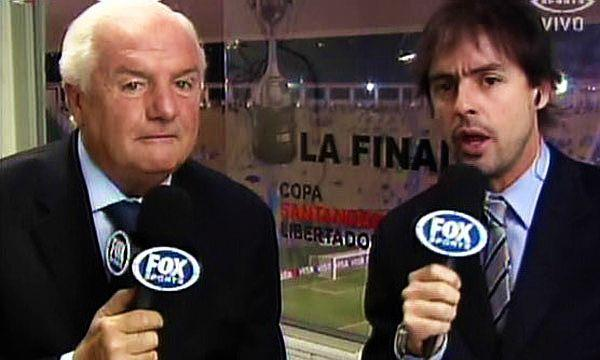
\includegraphics[scale=.3]{niembra.jpg}
\end{center}

\vskip 10pt
\hrule
\vskip 5pt

{\bf\noindent Introducci\'on}

Seg\'un se ha publicado en algunos medios deportivos de cuestionable credibilidad, el Comit\'e Ejecutivo de la Asociaci\'on de F\'utbol Argentina (AFA) quiere, con el fin de reconquistar los espacios de poder otrora ostentados, marcar tendencia en la incorporaci\'on de tecnolog\'ia de \'ultima generaci\'on para la resoluci\'on de situaciones conflictivas durante los partidos. Para ello se busca dar el primer paso mediante el desarrollo de un prototipo que permita decidir en tiempo real, mediante una imagen de la televisi\'on, si la pelota traspas\'o o no la l\'inea de gol. El objetivo ulterior de semejante empresa es destronar al sistema utilizado durante la Copa del Mundo 2014, principalmente por sus elevados costos de implementaci\'on y mantenimiento.

El Equipo de Desarrollos de M\'etodos Num\'ericos (EDMN) fue contactado para hacerse cargo del desaf\'io, teniendo en nuestras manos el futuro de un negocio millonario y, por qu\'e no, eventualmente la posibilidad de llegar nuevamente a la final de un mundial. Como propuesta, el prototipo en \emph{Fase 0} se basar\'a en la utilizaci\'on de t\'ecnicas de interpolaci\'on aplicadas al procesamiento de se\~nales, en particular para el re-escalamiento de im\'agenes de alta definici\'on.\\

\vskip 5pt

{\bf\noindent Definici\'on del problema y metodolg\'ia}

Para resolver el problema planteado en la secci\'on anterior, se considera el siguiente contexto. Dada una imagen de $m \times n$, con  $i = 1,\dots,m$ y $j = 1,\dots,n$, en escala de grises, se busca obtener un re-escalamiento de la misma de un factor $f$ predeterminado de antemano. En particular, consideraremos solamente agrandar la imagen, tomando $f > 1$, y para simplificar algunas cuestiones t\'ecnicas menores asumiremos que recibimos como par\'ametro un n\'umero $k \in \mathbb{N}_{>0}$ que denota la cantidad de filas (columnas) que ser\'an agregadas entre dos filas $i$ e $i+1$, $i = 1,\dots,m-1$ (columnas $j$ y $j+1$) de la imagen original. Luego, el ratio $f$ quedar\'a autom\'aticamente determinado por el cociente $\frac{(k+1)*(m-1) + 1}{m}$. Las figuras \ref{fig:imgorig} y \ref{fig:imgnew} muestran la transformaci\'on sobre un ejemplo correspondiente a una imagen de $3 \times 3$ y tomando $k = 2$.


\begin{figure}[!h]
%\begin{subfigure}[c]{0.45\textwidth}
\begin{center}
	\begin{tikzpicture}
    	\fill[red!20](0,0) rectangle (3,3); 
	  	\draw (0,0) grid (3,3);
		\setcounter{row}{1}
		\setrow {1}{2}{3}
		\setrow {4}{5}{6}
		\setrow {7}{8}{9}
	\end{tikzpicture}
\caption{Imagen original}
\label{fig:imgorig}
\end{center}
%\end{subfigure}
\end{figure}
\begin{figure}[!h]
%\begin{subfigure}[c]{0.45\textwidth}
\begin{center}
	\begin{tikzpicture}
    	\fill[red!20](0,0) rectangle (1,1); 
    	\fill[gray!20](0,1) rectangle (1,2); 
    	\fill[gray!20](0,2) rectangle (1,3); 
    	\fill[red!20](0,3) rectangle (1,4); 
    	\fill[gray!20](0,4) rectangle (1,5); 
    	\fill[gray!20](0,5) rectangle (1,6); 
    	\fill[red!20](0,6) rectangle (1,7); 
		\fill[gray!20](1,0) rectangle (2,7);
		\fill[gray!20](2,0) rectangle (3,7);
    	\fill[red!20](3,0) rectangle (4,1); 
    	\fill[gray!20](3,1) rectangle (4,2); 
    	\fill[gray!20](3,2) rectangle (4,3); 
    	\fill[red!20](3,3) rectangle (4,4); 
    	\fill[gray!20](3,4) rectangle (4,5); 
    	\fill[gray!20](3,5) rectangle (4,6); 
    	\fill[red!20](3,6) rectangle (4,7); 
		\fill[gray!20](4,0) rectangle (5,7);
		\fill[gray!20](5,0) rectangle (6,7);
    	\fill[red!20](6,0) rectangle (7,1); 
    	\fill[gray!20](6,1) rectangle (7,2); 
    	\fill[gray!20](6,2) rectangle (7,3); 
    	\fill[red!20](6,3) rectangle (7,4); 
    	\fill[gray!20](6,4) rectangle (7,5); 
    	\fill[gray!20](6,5) rectangle (7,6); 
    	\fill[red!20](6,6) rectangle (7,7); 
	  	\draw (0,0) grid (7,7);

		\setcounter{row}{1}
		\setrowaux {1}{}{}{2}{}{}{3}
		\setrowaux {}{}{}{}{}{}{}
		\setrowaux {}{}{}{}{}{}{}
		\setrowaux {4}{}{}{5}{}{}{6}
		\setrowaux {}{}{}{}{}{}{}
		\setrowaux {}{}{}{}{}{}{}
		\setrowaux {7}{}{}{8}{}{}{9}
	\end{tikzpicture}
\end{center}
\caption{Imagen re-escalada}
\label{fig:imgnew}
%\end{subfigure}
\end{figure}

El problema a resolver consiste en determinar cómo rellenar los casilleros grises, es decir, aquellos que no contienen la informaci\'on original de la imagen. Para ellos, se propone considerar al menos los siguientes tres m\'etodos:

\begin{enumerate}
\item \emph{Vecino m\'as cercano:} Consiste en rellenar aquellas posiciones correspondientes a nuevos p\'ixeles replicando los valores de alguno de los p\'ixeles que se encuentran en un vecindario de la posici\'on en consideraci\'on. \label{item:nn}
\item \emph{Interpolaci\'on bilineal:} Consiste en rellenar los p\'ixeles utilizando interpolaciones lineales entre p\'ixeles consecutivos de la imagen original, primero completando aquellas posiciones correspondientes a filas y columnas con informaci\'on original de la imagen y, luego, rellenando el resto. Tambi\'en es posible interpretar el m\'etodo como uno de dos fases, donde primero se aplica sobre las filas y luego, sobre la matriz resultante, se aplica por columnas (o viceversa). \label{item:bilineal}
\item \emph{Interpolaci\'on por Splines:} Simliar al anterior, pero considerando interpolar utilizando splines y tomando una cantidad de p\'ixeles mayor. Una alternativa a considerar es tomar la informaci\'on de bloques de un tama\~no fijo (por ejemplo, $4\times 4, 8\times 8,$ etc.), con el tama\~no de bloque a ser determinado experimentalmente. \label{item:spline}
\end{enumerate}

\newpage

Cada m\'etodo tienen sus propias caracter\'isticas, ventajas y desventajas particulares. Para realizar un an\'alisis cuantitativo, llamamos $I$ a la imagen real (ideal) que deber\'iamos obtener con nuestro algoritmo, y sea $\bar{I}$ la imagen efectivamente reconstruida. Consideramos entonces dos medidas, directamente relacionadas entre ellas, como el \emph{Error Cuadr\'atico Medio} (ECM) y \emph{Peak to Signal Noise Ratio} (PSNR), denotados por $\texttt{ECM}(\bar{I})$ y $\texttt{PSNR}(I)$, respectivamente, y definidos como:
\begin{equation}
\texttt{ECM}(I,\bar{I}) = \frac{1}{mn}\sum_{i=1}^m\sum_{j = 1}^n |I_{ij} - \bar{I}_{ij}|^2 \label{eq:ecm}
\end{equation}
\noindent y
\begin{equation}
\texttt{PSNR}(I,\bar{I}) = 10 \log_{10}\bigg(\frac{255^2}{\texttt{ECM}(I,\bar{I})}\bigg). \label{eq:psnr}
\end{equation}

En conjunto con los valores obtenidos para estas m\'etricas, es importante realizar un an\'alisis conjunto el tiempo de ejecuci\'on de cada m\'etodo y los denominados \emph{artifacts} que produce cada uno de ellos. Se denomina \emph{artifact} a aquellos errores visuales resultantes de la aplicaci\'on de un m\'etodo o t\'ecnica. La b\'usqueda de este tipo de errores complementa el estudio cuantitativo mencionado anteriormente incorporando un an\'alisis cualitativo (y eventualmente subjetivo) sobre las im\'agenes generadas.

\vskip 5pt

{\bf\noindent Enunciado}

Se pide implementar un programa en \verb-C- o \verb-C++- que implemente como m\'inimo los tres m\'etodos mencionados anteriormente, y que dada una imagen y un valor $k$ aplique estas t\'ecnicas para re-escalar la misma. A su vez, es necesario explicar en detalle c\'omo se utilizan y aplican los m\'etodos descriptos en \ref{item:nn}, \ref{item:bilineal} y \ref{item:spline} en el contexto propuesto. Los grupos deben a su vez plantear, describir y realizar de forma adecuada los experimentos que consideren pertinentes para la evaluaci\'on de los m\'etodos, justificando debidamente las decisiones tomadas y analizando en detalle los resultados obtenidos. Sumado a los experimentos planteados para la evaluaci\'on de los m\'etodos, se pide que cada grupo utilice al menos dos casos de prueba con im\'agenes de una resoluci\'on considerable (digamos, mayor a $1024\times 1024$ o $2048\times 2048$ como m\'inimo).

El formato de archivos, la modalidad de ejecuci\'on y el esquema de experimentaci\'on queda abierto a elecci\'on de cada grupo, siendo extremadamente importante elegir un formato adecuado y, adem\'as, proveer en la entrega una descripci\'on detallada con las instrucciones para la ejecuci\'on del programa y los pasos a seguir para replicar los experimentos realizados. Adem\'as, se debe incluir un ap\'endice donde se detalle c\'omo evaluaron la correctitud de toda la implementaci\'on.

\vskip 0.5 cm
\hrule
\vskip 0.2 cm

{\bf Sobre la entrega}
\begin{itemize}
\item \textsc{Formato electr\'onico:} Domingo 21 de Junio de 2015, {\bf{\underline{hasta las 11:59am}}}, enviando el trabajo
(\texttt{informe} + \texttt{c\'odigo}) a \texttt{metnum.lab@gmail.com}. El \texttt{asunto} del email debe comenzar con el texto \verb|[TP3]| seguido
de la lista de apellidos de los integrantes del grupo. Ejemplo: \texttt{[TP3] Acevedo, Miranda, Montero}
\item \textsc{Formato f\'isico:} Lunes 22 de Junio de 2015, en la clase pr\'actica.
\end{itemize}


\end{document}